% LaTeX hjelpedokument for TFE4101
% Laget av Sveinung Haugane, vår 2019.

% Dette er en kommentar. Alt som følger en "%" er ikke en del av det kompilerte dokumentet.

% \documentclass[<options>]{<dokumenttype>} bestemmer hvordan layouten på sidene skal være.
% For labrapporten bruker vi article, som gjør at grunnformateringen er lik for hver side. 
% Et annet alternativ er book, som gjør at layouten blir som en innbundet bok.
% Det er også her vi setter skriftstørrelse, papirstørrelse, tosidig print layout etc.
\documentclass[12pt, a4paper]{article}

% LaTeX er basert rundt å benytte pakker for å ta i bruk annen funksjonalitet.
% Pakker inkluderes ved å benytte \usepackage[<package options>]{<package name>}.
% Dere kommer ikke unna bruk av pakker, hvis dere ønsker å bruke LaTeX effektivt.
% Pakken geometry gir mange fler valg for å sette marger og sidelayout.
\usepackage[lmargin=25mm,rmargin=25mm,tmargin=27mm,bmargin=30mm]{geometry}

% Bestemmer hvilken enkoding som benyttes for input fra keyboard. Anbefaler utf8.
% Dere vil da mest sannsynlig ikke få problemer med æøå.
\usepackage[utf8]{inputenc}

% Fontenc styrer fonten som blir brukt. T1 fungerer fint.
\usepackage[T1]{fontenc}

% Sett inn ekstern fil i hoveddokument.
% Legger inn en del pakker jeg kan anbefale å bruke.
% Det blir desverre for mye arbeid å forklare alle i detalj.
% De aller fleste Latex-pakker er godt dokumentert på nett.

% Babel definerer standard autogenerert tekst for mange forskjellige språk.
% Når vi senere kommer til figurtekst og lignende, vil dere se at Babel forsikrer
% at det står Figur og ikke Figure i den genererte figurteksten. Det samme gjelder
% for innholdsfortegnelse etc.
\usepackage[norsk]{babel}

% << >> erstatter "" i referanseliste (Frivillig)
\usepackage{csquotes}

% Gjør at output PDF støtter linker.
\usepackage[hidelinks]{hyperref}

% For mer fleksible nummererte lister.
\usepackage{enumitem}

% Definerer de aller fleste mattesymboler. Feks. Integrasjonstegn, Sum, XOR osv.
\usepackage{amsmath}

% For å inkludere bilder i rapporten. Takler ganske mange formater
\usepackage{graphicx}
% Søkepath for å finne bilder. Dette er alternativt til å skrive full path der dere legger inn bildet.
\graphicspath{{./figurer/}}
\usepackage{subcaption}

% Brukes for å få tekst til å gå over flere rader i en tabell.
\usepackage{multirow}

% Hovedpakke for tikz figurtegning
\usepackage{tikz}
% Utvidelse for 3D-tegning
\usepackage{tikz-3dplot}
\usetikzlibrary{shapes, arrows}
% Utvidelse for kretstegning. Kun denne er nødvendig for kretstegning.
\usepackage[siunitx]{circuitikz}

% En av pakkene som kan brukes til referanser
\usepackage[style=ieee, citestyle=numeric-comp]{biblatex}
\addbibresource{mylib.bib}

% PDF som appendiks
\usepackage{pdfpages}

% De to linjene nedenfor sikrer at nye avsnitt ikke starter med tab, og at det blir 
% mellomrom mellom avsnittene. Dere skal få styre dette selv, men personlig liker jeg
% innstillingen nedenfor.
\setlength\parindent{0pt}
\setlength{\parskip}{1em}

% Hele dokumentets innhold defineres i rekkefølge mellom \begin{document} og 
% \end{document} (titlepage og noen andre ting er spesielle tilfeller)
\begin{document}

% Det som skal på rapportens forside kan defineres innenfor et titlepage scope.
% Linjeskift kan tvinges frem med dobbel backspace \\ eller tom kodelinje.
% Titlepage blir ikke nummerert.
\begin{titlepage}
    % Tekst i mellom \begin{center} og \end{center} blir sentrert. 
    \begin{center}
        % \vspace{<lengde>} setter hvor mye whitespace som skal være i mellom linjene. 
        % For å sette mellomrom relativt til marg, må man benytte \vspace*{<lengde>}
        \vspace*{1.5cm}
        % Sjekk denne for å se på tekststørrelser: https://texblog.org/2012/08/29/changing-the-font-size-in-latex/
        {\Huge\textbf{Labrapport Lab 3: RC-Krets og CMOS logikk}}\\
        \vspace{1cm}
        {\Large av Arran Kostveit Gabriel og Stefan Mack}\\
        \vspace{1cm}
        \today\\ % Setter inn dagens dato ved kompilering
        \vspace{1cm}
        Labgruppe 24, pulje 3\\
        
        %\vfill fyller siden med whitespace, slik at teksten som følger havner neders.
        %\hfill gjør tilsvarende horisontalt.
        \vfill
        {
            \large TFE4101 Krets og Digitalteknikk\\ 
            Norges Teknisk-Naturvitenskapelige Universitet
        }
        
        
        
    \end{center}
\end{titlepage}

% \pagenumbering velger automatisk sidenummereringsstil.
%   - gobble (ingen nummerering)
%   - arabic (normal nummerering)
%   - roman (romerske tall)
\pagenumbering{roman}

% \Clearpage sier at det som kommer på de følgende linjene skal starte på neste side.
\clearpage

% For oversikten sin del kan man med fordel dele opp teksten i flere underdokumenter.
% For å sette et dokument inn i hoveddokumentet brukes \input{</path/to/filnavn.tex>}
% Hvis det ligger i samme mappe som hoveddokumentet trengs ingen spesiell path.
\section{Sammendrag}

    Denne rapporten tar for seg to forsøk  som ble gjennomdørt under laboratorieøving 3 i TFE4101. Det første forsøket gikk ut på å gjennomføre målinger av en RC-krets ved hjelp av oscilloskop.
    Med hensikt å analysere en kondensators effekt på et AC signal.
    Det andre forsøket gikk ut på å analysere en CMOS-krets med forskjellige inngangssignaler;
    CMOS er en innfallsvinkel for å utvikle digitale kombinatoriske kretser. Hensikten med det andre forsøket vundersøke de elektriske egenskapene til en CMOS-krets

    Kondensatoren i RC-Kretsen hadde en dempende effekt på den oscillerende spenningen fra signal generatoren. Det vil kunne være mulig å annvende dette til å stabilisere et analogt signal for å fjerne støy. En annen mulig annvendelse er en AC til DC transformator

    Spenningen i CMOS kretsen varierte selv for signaler som skal tolkes som samme binære verdi. En modell som annser logiske porter som perfekte matematiske funksjoner vil være en grov approksimasjon og kan i enkelte tilfeller medføre feile estimasjoner. Dette kommer fra at logiske kretser i bunn består av elektriske komponenter, som ikke er matematisk perfekte, uten motstand, og upåvirket av utvendige faktorer. \clearpage

% \tableofcontents setter inn automatisk generert innholdsfortegnelse.
% Hva som vises her er bestemt av kapitteloverskriftene. Kommer tilbake til dette.
\tableofcontents
\addcontentsline{toc}{section}{Innhold}
\clearpage
\pagenumbering{arabic}
\setcounter{page}{1}

\section{Innledning}

I denne rapporten skriver vi om mye

Skriv generelt om hva laboppgaven handler om, at det er en del av labopplegget i TFE4101 på NTNU. 
Dere kan også skrive om rapportens struktur, hvis det er noe spesielt dere ønsker å få fram.

\subsection{Figurer}

Det finnes flust av måter å lage figurer på i latex. For å legge inn bilder er pakken graphicx brukt mest. En figur dannes innenfor et figure scope. 
Vi ser i figur~\ref{fig:inl_6cm_pika} en 6cm høy pikachu opp ned. Denne skiller seg ut fra Pikachu i figur~\ref{fig:inl_scaled_pika}~og~\ref{fig:inl_relative_pika}, som er en del av figur~\ref{fig:inl_subfigs_main}.

% OBS til avsnittet over
% ~ Brukes til å forsikre seg om at det havner på samme linje.


% \begin{figure}[<placement specifier>]
% Plassering i LaTeX kan være knotete, og er antagelig noe av det dere kommer til å bruke mest tid på.
% De vanligste er:
%   - h (plasser her i teksten)
%   - t (plasser på toppen av neste side
%   - b (plasser på bunn av denne siden)
%   - ! (Få kompilatoren til å bry seg mer om disse plasseringsegenskapene enn feks marger)
% ! fungerer ikke alene, og kommandoene er i prioritert rekkefølge fra venstre til høyre.
\begin{figure}[!htb]
    %\centering gjør at alt som følger innenfor dette scopet sentreres
    \centering
    
    % Sett inn grafikkfil \includegraphics[<formatering>]{<path/to/file.extension>}
    
\includegraphics[height=6cm, angle=180]{figurer/pika.jpg}
    \caption{6cm høy Pikachu}
    \label{fig:inl_6cm_pika}
\end{figure}

\begin{figure}[!htb]
    \centering
    % Subfigure er definert i pakken subcaption.
    % bruk: \begin{subfigure}{<størrelse figurområde>}
    % \textwidth er en innebygd størrelse basert på margene på siden.
    % 0.45\textwidth betyr: Denne underfiguren tildeles 45% tilgjengelig sidebredde for tekst.
    % Dette er alltid relativt til avsatt plass. Legg spesielt merke til width=0.9\linewidth
    % i subfigur nr 2.
    \begin{subfigure}{0.45\textwidth}
        \centering
        
\includegraphics[scale=0.15]{figurer/pika.jpg}
        % \caption er figurtekst. Må komme før \label
        \caption{Skalert Pikachu}
        % \label er figurreferanse til bruk for referering. Må etter \caption
        \label{fig:inl_scaled_pika}
    \end{subfigure}
    \begin{subfigure}{0.45\textwidth}
    \centering
        
\includegraphics[width=0.9\linewidth]{figurer/pika.jpg}
        \caption{Størrelse er relativt til linjebredde}
        \label{fig:inl_relative_pika}
    \end{subfigure}

    % Ytterste figurtekst of referansenivå.
    \caption{Hovedfigur}
    \label{fig:inl_subfigs_main}
\end{figure}

\clearpage

\subsection{Tabeller}

For å sette inn en tabell brukes table environment Her kan jeg anbefale å bruke tabular for å lage selve tabellen. 
Tabell~\ref{tab:inl_full_tabell} viser tekstjustering, tabell~\ref{tab:inl_sparse_tabell} viser et annet linjeoppsett,
og tabell~\ref{tab:inl_multi_tabell} viser multikolonner og rader.

% \begin{table}[<placement>]
\begin{table}[!htb]
    \centering
    \caption{Vanlig tabell}
    \label{tab:inl_full_tabell}
    
    % Tabular lager selve tabellen. Defineres ved \begin{tabular}{<radformattering>}
    % | betyr vertikal linje, c, l, r er tekstjustering.
    % I tabeller skilles hvert radelement med &. 
    % Ny linje legges inn med \\
    \begin{tabular}{|c|l|r|}
        %horisontal linje \hline. 
        \hline
        \textbf{Sentrert}   & \textbf{venstrejustert}   & \textbf{høyrejustert} \\ \hline \hline
         hei                & på                        & deg                   \\ \hline 
    \end{tabular}
\end{table}

\begin{table}[!htb]
    \centering
    \caption{Tabell med mindre inndeling}
    \label{tab:inl_sparse_tabell}
    \begin{tabular}{c|c}
        \textbf{Vare}   & \textbf{Verdi} \\ \hline
        Vann            & 3kr \\
        Mer vann        & 4kr \\
        Masse vann      & 12kr \\ \hline
        Sum             & 19kr \\
    \end{tabular}
\end{table}

% Tabeller med mye formattering kan ofte bli uoversiktlige desverre. 
% Bruk tabs for å lage oversikt.
% For multirad bruk \multirow{<antall>}{<bredde>}{<tekst>}
% For multikolonne bruk \multicolumn{<antall>}{<formattering>}{<tekst>}
\begin{table}[!htb]
    \centering
    \caption{multirad og multikolonne}
    \label{tab:inl_multi_tabell}
    \begin{tabular}{|c|c|c|} 
        \hline
        \multicolumn{3}{|c|}{\textbf{Felles overskrift}} \\ \hline
        \multirow{4}{3cm}{\centering Valg}  & Ja &  \\ \cline{2-3}
                                            & Nei & \\ \cline{2-3}
                                            & Kanskje & X \\ \cline{2-3}
                                            & Vet ikke & \\ \hline
    \end{tabular}
\end{table}\clearpage

\section{Innledning og Teori}

\subsection{Kondensatorer og RC kretser}

    \begin{itemize}
        \item[-] Kondensator: En kondensator er en passiv elektrisk komponent viss bruksområde er å lagre elektrisk ladning.
        Den består av to elektroder skilt med et dielektrisk materiale.
        Et dielektrisk materiale har elektrisk isolerende egenskaper og polariseres når det påvirkes av et elektrisk felt.
        Kondensatorer beskrives symbolsk ved likningen \ref{eq:farads}.
        \begin{equation}
            F = \frac{Q}{U}
            \label{eq:farads}
        \end{equation}
        I likning \ref{eq:farads} er $Q$ ladning målt i Coulomb, $U$ er spenning målt i Volt og $F$ er kapasitansen målt i Fahrrad.
        Fahrrad tilsvarer altså Coulomb/Volt.
        Kapasitansen beskriver mengden elektroner som må tilføres elektrodene for å danne en gitt spenning over dem.
        \item[-] RC-Krets: En enkel RC-krets består av en motstand og en kondensator koblet i serie se figur (3-1 ish).
        Spenning over kondensatoren i en slik krets kan beskrives ved \ref{eq:rc-oppladning} under oppladning og \ref{eq:rc-utladning} under utladning.
        \begin{equation}
            v_{C}(t) = V_{kilde} \cdot \left( 1 - e^{-\frac{t}{\tau}} \right)
            \label{eq:rc-oppladning}
        \end{equation}
        \begin{equation}
            v_{C}(t) = V_{kilde} \cdot e^{-\frac{t}{\tau}}
            \label{eq:rc-utladning}
        \end{equation}
        Begge er uttrykt ved tiden $t$ gitt i sekunder, og gjelder for $t \geq 0$.
        $\tau = R \cdot C$, $R$ er motstand målt i Ohm, og $C$ er kapasitans målt i Fahrrad.
        % TODO source formulas
    \end{itemize}

\subsection{Transistorer}

    \begin{itemize}
        \item[-] PMOS-, og NMOS-transistor: De mest grunnleggende byggeklossene i logiske kretser er disse to formene for transistor, som begge fungerer som brytere.
        PMOS slipper signaler gjennom ved input: lav, og blokkerer dem ved input: høy.
        NMOS fungerer på samme måte, men invertert.
        Se figur~\ref{fig:pnmos_transistors} Ved bruk av disse kan man konstruere alle logiske porter.
        \item[-] NAND port: En to-inngangs NAND port er en logisk port som tar to binære input signaler og utfører funksjonene NOT og AND på dem for å produsere ett output signal.
        Se figur~\ref{fig:tt_nand} for sannhetstabellen til NAND porten.
        Se figur~\ref{fig:NAND_transistorlevel} for oppbyggingen av en NAND port med bruk av PMOS-, og NMOS-transistorer.
        \item[-] Kombinatorisk CMOS-logikk: En CMOS krets består av en eller flere logiske porter bygget på PMOS-, og NMOS-transistorer.
    \end{itemize}

    \begin{figure}[!htb]
        \centering
        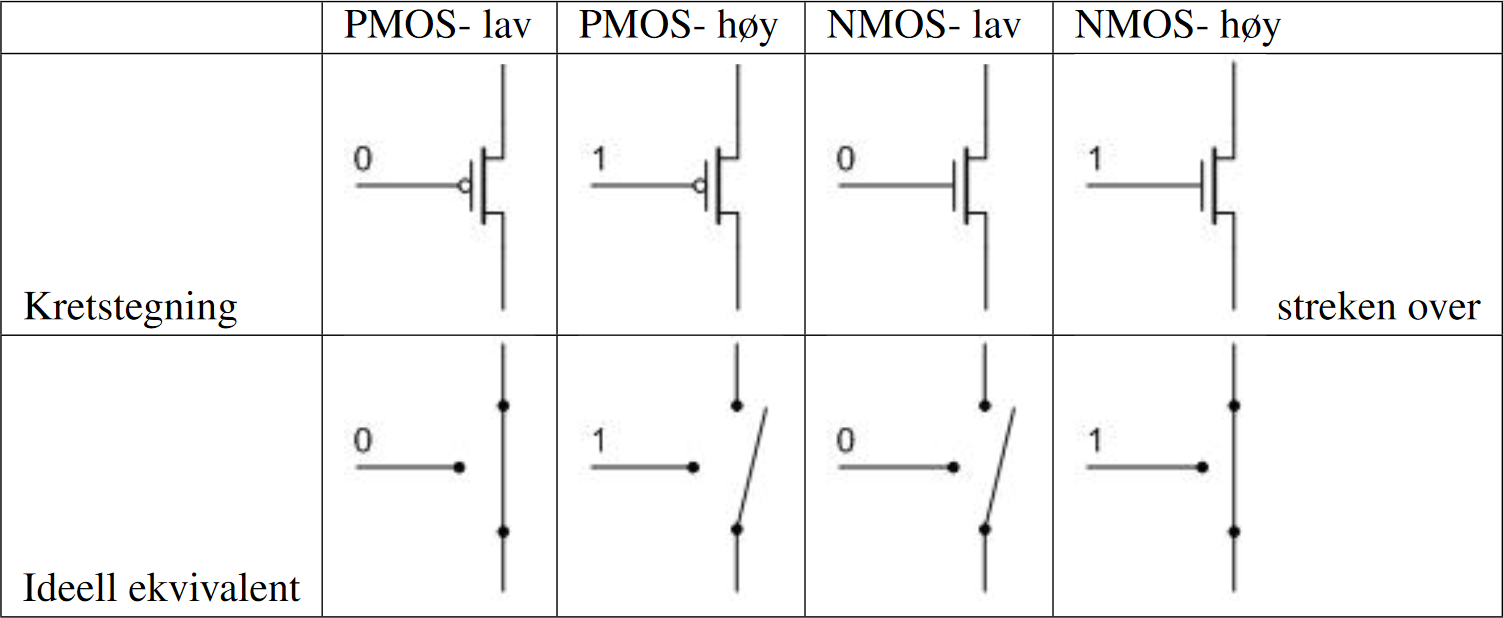
\includegraphics[height=4cm]{figurer/PNMOS.png}
        \caption{PMOS og NMOS- transistor med deres ideelle ekvivalenter for åpen og lukketkanal.}
        \label{fig:pnmos_transistors}
        ~\cite{labhefte}
    \end{figure}

    \begin{figure}[!htb]
        \centering
        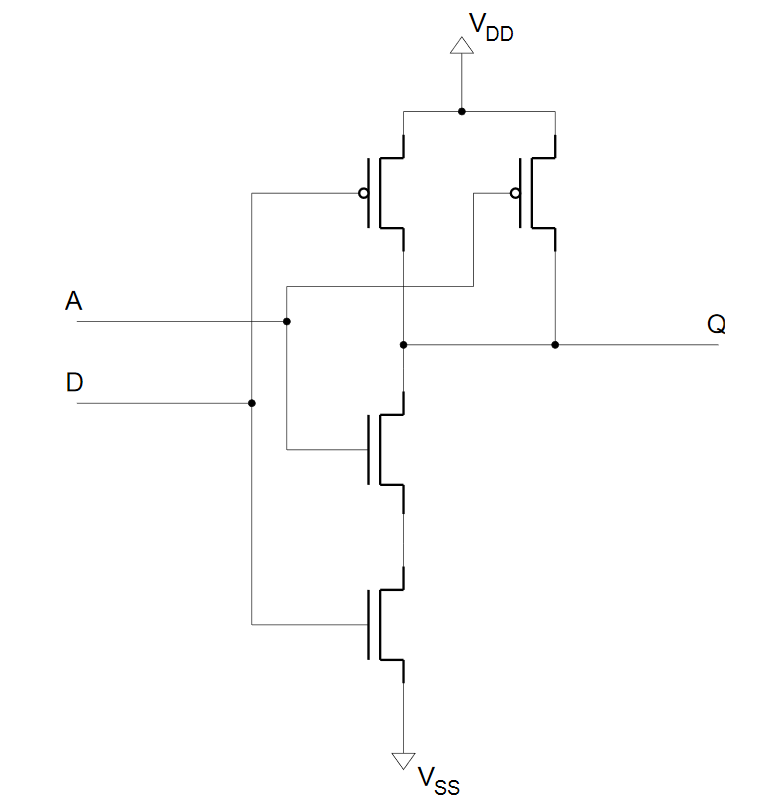
\includegraphics[height=8cm]{figurer/NAND_transistorlevel.png}
        \caption{NAND port på transistornivå.}
        \label{fig:NAND_transistorlevel}
        ~\cite{labhefte}
    \end{figure}

    \begin{figure}[!htb]
        \centering
        \begin{tabular}{|c|c|c|}
            \hline
            \textbf{A} & \textbf{B} & \textbf{A NAND B} \\ \hline
            0 & 0 & 1 \\
            0 & 1 & 1 \\
            1 & 0 & 1 \\
            1 & 1 & 0 \\ \hline
        \end{tabular}
        \caption{Sannhetstabell for NAND port}
        \label{fig:tt_nand}
    \end{figure}\clearpage

\section{Gjennomføring}

Gjennomføringen deles i to hoveddeler, RC-Krets og CMOS logikk. De to arbeidene er uavhengige av hverandre. 
Ved porter refereres det til inngangene på veroboard sokkel, som samsvarer med de nederst på kretskort figuren i appendiks L

\subsection{RC-Krets}

\subsubsection{Lodding}
Først ble kretsen, som beskrevet i Figur \ref{fig:rc}, loddet på kretskortet. En $1k\Omega$ motstand ble loddet på posisjon $R_{10}$, og en 15nF kondensator ble loddet på posisjon $C_{1}$

\begin{figure}[!htb]
    \centering
    \begin{circuitikz}
        \draw
            (0,0) to [vsourcesquare] (0,5)
            to [european resistor] (10,5)
            to [capacitor] (10,0) -- (0,0)
        ;
        \draw[fill] (0,5) circle [radius=0.1];
        \draw[fill] (10,5) circle [radius=0.1];
        \draw[fill] (10,0) circle [radius=0.1];
        \draw[fill] (0,0) circle [radius=0.1];
        \node [above] at (5,4) {$R_{10}=1k\Omega$};
        \node [above left] at (10,1) {$C_{1}=1nF$};
        \node [above left] at (0, 1) {$Sig.gen=(0,4)V$};
    \end{circuitikz}
    \caption{RC-Krets}
    \label{fig:rc}
\end{figure}

\subsubsection{Signalgenerator}
Signalgeneratoren ble stilt inn slik at den sendte ut en firkantpuls med frekvens på 3 KHz og amplitude på 4V, med 2V i offset slik at signalet har toppunkt i 4V og bunnpunkt i 0V.

\subsubsection{Måling}
\label{subsec:rc-maaling}
Signalgeneratoren, ved hjelp av et T-ledd, ble så koblet til både kretsen via veroboardet (port 19 og port 17), og til oscilloskopet. Ved å måle spenningen over kondensatoren vc (port 18 og port 17) og spenningen fra generatoren på forskjellige kanaler var det mulig å se både spenningen som signalgeneratoren påtrykte, og hvordan spenningen endret seg etter å ha gått gjennom kondensatoren. 
$\tau$ ble også målt, dette ved å plassere en "cursor"\ på det punktet der kondensatoren var ladet 2/3 i oscilloskopet og lese av tiden det tok for kondensatoren å nå det punktet.

\newpage % bruk denne for å starte en ny side.
\subsection{CMOS logikk}

\subsubsection{Lodding}
Først ble kretsen, som beskrevet i Figur \ref{fig:lg}, loddet opp på kretskortet, med verdier som anvist i figuren. I tillegg måtte strappingen S2 loddes inn for koblet sammen logikk kretsen og driver kretsen.


\begin{figure}[!htb]
    \centering
    \begin{circuitikz}
        % Draw components
        \draw (0,2) node[circ, scale=1.5] (A){A};
        \draw (0,1) node[circ, scale=1.5] (B){B};
        \draw (0,0) node[circ, scale=1.5] (C){C};

        \draw (1, -2) node[genericshape, rotate=90] (R4){$R_4=1.5M\Omega$};
        \draw (2, -2) node[genericshape, rotate=90] (R3){$R_3=1.5M\Omega$};
        \draw (3, -2) node[genericshape, rotate=90] (R2){$R_2=1.5M\Omega$};
        \draw (8, -2) node[genericshape, rotate=90] (R5){$R_5=4.7k\Omega$};
        \draw (9, 2) node[genericshape] (R6){$R_6=4.7k\Omega$};
        \draw (12, -2) node[genericshape, rotate=90] (R7){$R_7=4.7k\Omega$};

        \draw (1,0) node[circ, scale=1.5] (R4P){};
        \draw (2,1) node[circ, scale=1.5] (R3P){};
        \draw (3,2) node[circ, scale=1.5] (R2P){};
        \draw (2, -3) node[circ, scale=1.5] (JP){};
        \draw (8, 2) node[circ, scale=1.5] (GP){};
        
        \draw (2, -5) node[ground] (G){$V_{SS} - Jord$};
        \draw (8, -5) node[ground] (G2){$V_{SS} - Jord$};
        \draw (12, -5) node[ground] (G3){$V_{SS} - Jord$};

        \draw (12, 4) node[vcc] (vdd){$V_{DD}$};

        \draw (5,1) node[nand port] (nand1){};
        \draw (7,2) node[nand port] (nand2){};

        \draw (12, 2) node[npn] (npn){BC547C};

        \draw (12, -4) node[emptydiodeshape, rotate=-90] (diode){};

        % Draw lines
        \draw (C) -| (nand1.in 2);
        \draw (B) -| (nand1.in 1);
        \draw (A) -| (nand2.in 1);
        \draw (G) -- (JP);
        \draw (G2) -- (R5);
        \draw (R5) -- (GP);
        \draw (nand2.out) -- (GP);
        \draw (GP) -- (R6);
        \draw (R6) -- (npn);
        \draw (JP) -| (R4);
        \draw (JP) -| (R3);
        \draw (JP) -| (R2);
        \draw (R4) -- (R4P);
        \draw (R3) -- (R3P);
        \draw (R2) -- (R2P);
        \draw (npn.E) -- (R7);
        \draw (npn.C) -- (vdd);
        \draw (R7) -- (diode);
        \draw (diode) -- (G3);
        \draw (nand1.out) -| (nand2.in 2);
    \end{circuitikz}
    \caption{Logisk-Krets}
    \label{fig:lg}
\end{figure}

\subsubsection{Måling}
Det ble så målt spenningene til nodene D og Q på figur 2 med forskjellige inn-signaler på A, B, og C. 
Spenningene ble målt i fra jord (VSS). For å måle spenningen til node D ble proben til oscilloskop satt på port 9 (VSS) og port 4 på veroboard sokkelen. 
For node Q ble port 9 og port 5 brukt.\clearpage

\section{Resultater}

Resultatene fra begge forsøkene ble skrevet ned i labjournalen før den ble digitalisert

\subsection{RC-Krets}

Som Figur~\ref{fig:rc-resultater} viser hang spenningen over kondensatoren etter spenningen fra signalgeneratoren 

\begin{figure}[!htb]
    \centering
    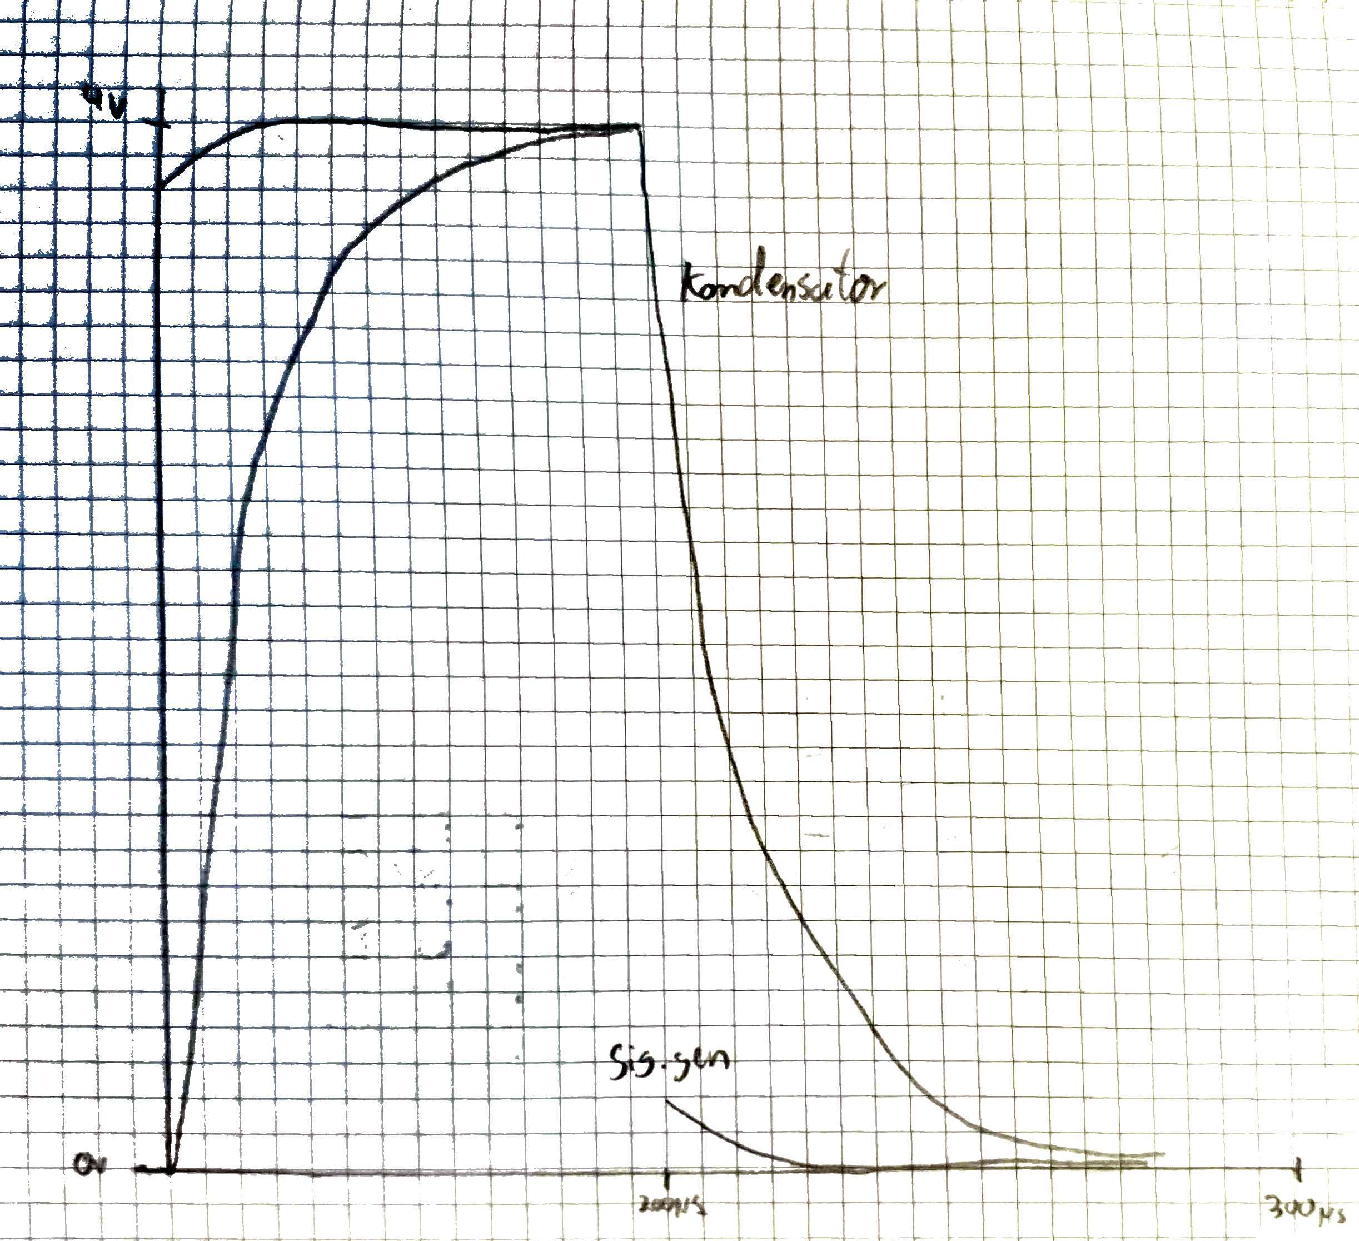
\includegraphics[height=6cm]{figurer/RC-figur.pdf}
    \caption{Spenningen over kondensatoren og signalgeneratoren}
    \label{fig:rc-resultater}
\end{figure}

Tisdkonstanten $\tau$ ble målt til å være $17\cdot 10^{-6}s$ ved prosedyren forklart i \ref{subsec:rc-maaling}

\subsection{CMOS logikk}

Figur~\ref{fig:cmos-resultater} viser spenningene målt ved punktene D og Q fra CMOS logikk kretsen som vist i Figur~\ref{fig:rc}. Målingene av D og Q er gjort i Volt.

\begin{figure}[!htb]
    \centering
    \begin{tabular}{|c|c|c|c|c|}
        \hline
        \textbf{A} & \textbf{B} & \textbf{C} & \textbf{D} & \textbf{Q} \\ \hline
        0 & 0 & 0 & 9 & 8.4 \\
        1 & 0 & 0 & 9 & 0 \\
        1 & 1 & 0 & 9 & 0 \\
        1 & 0 & 1 & 9 & 0 \\
        1 & 1 & 1 & 0 & 0 \\
        0 & 0 & 1 & 9 & 8.4 \\
        0 & 1 & 0 & 9 & 8.4 \\
        0 & 1 & 1 & 0 & 8.7 \\ \hline
    \end{tabular}
    \caption{Målingene av CMOS spenningene}
    \label{fig:cmos-resultater}
\end{figure}\clearpage

\section{Diskusjon}

\subsection{Diskusjon del 1.}

    Tau ble målt til $17 \cdot 10^{-6} \Omega F$, målingen viser et avvik fra det teoretiske $15 \cdot 10^{-6} \Omega F$ på ca $13.4$ prosent.
    Dette er ikke oppsiktsvekkende, da målemetoden vår delvis baserte seg på et øyemål på oscilloskopet.
    Videre avvikskilder kan svare til avvik i verdier fra komponentspesifikasjonene (se appendiks G) og motstand i ledninger ol.
    Som forventet av teorien viser målingene~\ref{fig:rc-resultater} at spenningen over kondensatoren ikke direkte følger spenningskilden, men er en demping av den over tid.
    Kondensatoren virker altså som en motstand mot endring i spenningen i kretsen.
    Konsekvensene av dette er mange, kondensatorer kan for eksempel brukes til å filtrere høyfrekvent støy i et analogt signal.
    Ettersom kondensatorer motstår momentane endringer i spenning vil høyfrekvente spenningsendringer kun føre til små endringer i den totale spenningen.
    Et annet bruksområde er konvertering mellom AC-, og DC-strøm.
    Vår enkle RC krets kan sees på som at den ‘skviser’ firkantpulssignalet sammen mot likevektslinjen, i dette tilfellet to volt, og med en høyere kapasitans (eller motstand) vil denne ‘skvisefaktoren’ blitt sterkere, og trende spenningen mot likevektslinjen.
    Vi kan tenke oss at dersom RC går mot uendelig går spenningen mot v0.

\subsection{Diskusjon del 2.}

    Resultatene av målingene av den kombinatoriske kretsen var som forventet, men det var en måling som stakk seg ut.
    Port Q er en NAND port og gav derfor output HØY når èn eller begge av inngangene stod på HØY.
    Allikevel måltes spenningen over Q høyere i det tilfellet der begge inngangene stod på LAV~\ref{fig:cmos-resultater}.
    Porter har intern motstand i transistorene de består av.
    Ved å analysere NMOS-transistorene i NAND-porten~\ref{fig:NAND_transistorlevel} som motstander finner vi forklaringen på avviket.
    Når kun ett av inngangssignalene står LAV går strømmen kun gjennom èn av NMOS-transistorene i porten, som kan sees ekvivalent med at spenningen fra driverkretsen (9V) påvirkes av en (liten) motstand.
    I det tilfelle der begge står LAV vil strømmen kunne gå gjennom begge NMOS-transistorene.
    % TODO legg til teorireferanse
    Vi vet fra teorien at motstander i parallell har mindre motstand enn den minste enkelt-motstanden, det er derfor naturlig at når begge inngangssignalene er LAV vil det være mindre spenningsfall, og derav høyere spenning over Q.

    På bakgrunn av dette oppstår det et problem med å tolke logiske kretser som rene modeller der man anser input og output til å være binære.
    Derfor oppgis det intervaller for logisk høy og logisk lav i spesifikasjoner for logiske porter.
    I vårt tilfelle var disse intervallene ca.\ $[-0.5V, 3V]$ for logisk lav og $[7V, 9.5V]$ for logisk høy (se appendiks G).
    Ca.\ da vi hadde $vdd=9V$ og ikke $10V$ som spesifisert i databladet.

    Det at en logisk krets på lavt nivå består av elektriske komponenter er det som medfører at signaler påvirkes av eksternt støy og interne faktorer.
    Dette viser til at det i virkeligheten ikke finnes digitale signaler.
    Men vi tillnærmer, med de unøyaktighetene som kan oppstå.
\clearpage

\section{Konklusjon}

Konklusjonen skal i bunn og grunn fortelle om dere fikk til det dere prøvde på, hvilke problemer og uforutsette problemer som kom underveis og hva som kunne vært forbedret. 
Konklusjonen fungerer også naturlig som en oppsummering av diskusjonsdelen.\clearpage

\printbibliography
\addcontentsline{toc}{section}{Referanser}
\clearpage

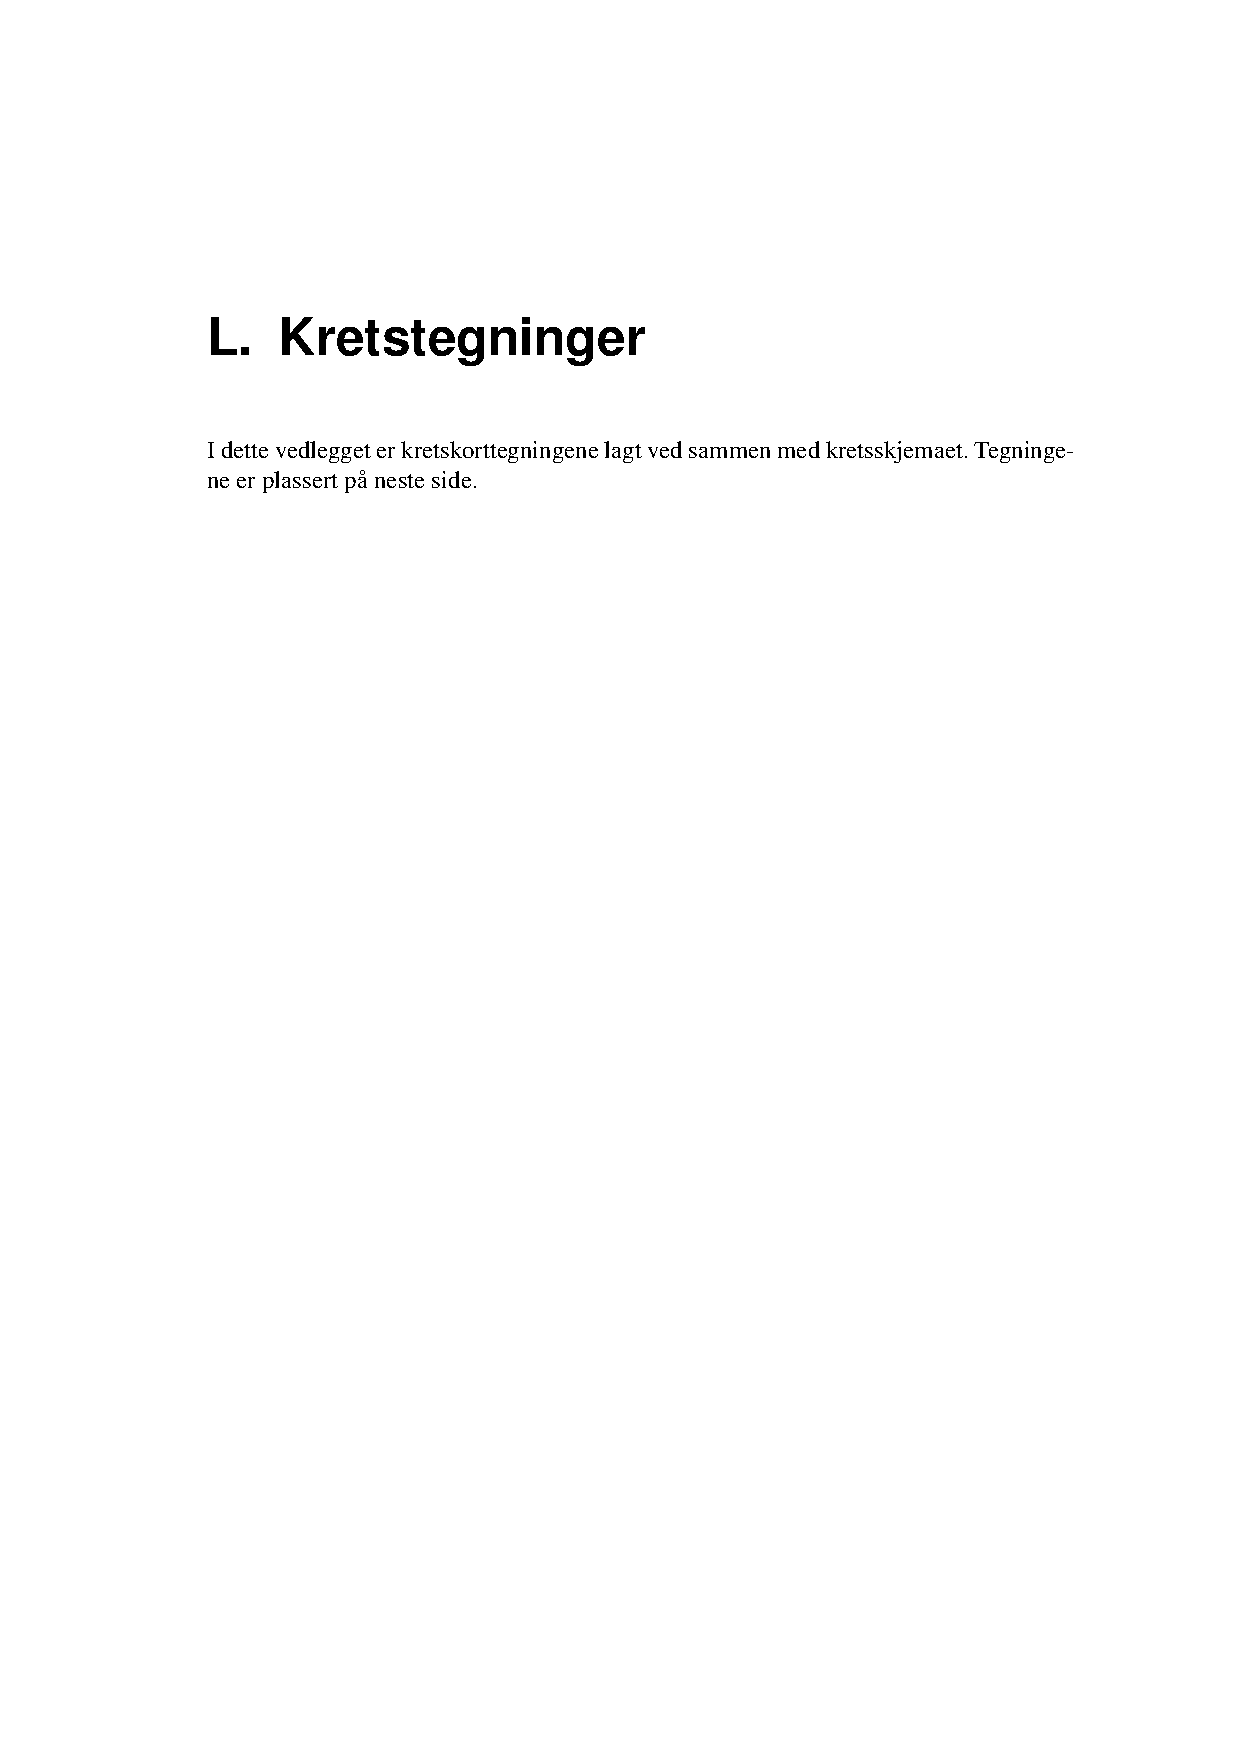
\includepdf[pages=-,pagecommand=\thispagestyle{plain}]{appendixL.pdf}

\end{document}
